\section*{Cycle 1 Experiment 4}

\section{\Large{Pipes, Message Queues and Shared Memory}}

\subsection{Aim}
\large To implement programs for Inter Process Communication using PIPE, Message Queue and Shared Memory.
\begin{itemize}
    \item Write a program for communication between a child process and its parent process with the use of Ordinary Pipes.
    \item Program to show IPC using Named pipes.
    \item Program to show IPC with the help of message queue. Here there are two processes- writer and reader.
    \item Program to show IPC with the help of shared memory. Here there are two processes- writer and reader.
\end{itemize}

\subsection{Theory}
\subsubsection*{\large Pipes}
Pipe is a communication medium between two or more related or interrelated processes. It can be either within one process or a communication between the child and the parent processes, or even be multi-level such as communication between the
parent, child, grand-child, etc. Two common types of pipes used on both UNIX and Windows systems: ordinary pipes and named pipes.\\
\\
\textbf{Ordinary Pipes: }Ordinary pipes allow two processes to communicate in a producer consumer fashion where the producer writes to one end of the pipe and the consumer reads from the other end. They are unidirectional. On UNIX systems, ordinary pipes are constructed using the function \\
\\
\textit{pipe(int fd[ ])}, where \\
fd[0] is the read-end of the pipe, \\
and fd[1] is the write-end. 
\\
\\
The major limitation of an ordinary pipe is that they are always local, ie. they cannot be used for communication over a network.
\\
\\
\textbf{Named Pipes: }A named pipe is a more powerful communication tool as it can be bidirectional and does not require any parent-child relationship. Once a named pipe is established, several processes can use it for communication. A named pipe exists in the file system. After input-output has been performed by the sharing processes, the pipe still exists in the file system independently of the process, and can be used for communication between some other processes. In order to create a namped pipe we make use of the mkfifo() function. A FIFO special file is entered into the filesystem by calling it. Once we have created it, any process can open it for reading or writing from both ends.
\\
\\
\subsubsection*{\large Message Queues}
It is a component used for IPC, or for inter-thread communication within the same process. It makes use of a queue for messaging – the passing of control or of content. Message queue is a linked list of messages stored within the kernel and identified by a message queue identifier. Every message has a positive long integer type field, a non-negative length, and the actual data bytes (corresponding to the length), all of which are specified to msgsnd() when the message is added to a queue. A new queue is created or an existing queue opened by msgget(). New messages are added to the end of a queue by msgsnd() and are fetched from the queue by msgrcv(). We don’t have to fetch the messages in a first-in, first-out order. Instead, we can fetch messages based on their type field.
\subsubsection*{\large Shared Memory}
Shared memory is a component used in IPC, where two or more process can access the common memory. Here, communication is done via this shared memory where changes made by one process can be viewed by anther process. The function shmget()
is used to create and return an identifier for the shared memory segment. Before one can use a shared memory segment, we should attach to it using the function, shmat(). Ususally the memory address to be used is automatically chosen by the
OS. After this, we can use the memory segment for communication. When we are done with the shared memory segment, the program should detach itself from it using shmdt(). In order to destroy the shared memory segment, shmctl() is used.

\subsection{Program \& Output}
\subsubsection{Ordinary Pipes}
\begin{verbatim}
#include<stdio.h>
#include<unistd.h>
#include<stdlib.h>
#define size 16

char* msgA = "Message A";
char* msgB = "Message B";
char* msgC = "Message C";

int main(){
    char inbuf[size];
    int p[2], i;
    
    if(pipe(p) < 0)
        exit(1);
    write(p[1], msgA, size);
    write(p[1], msgB, size);
    write(p[1], msgC, size);
    for(i = 0; i < 3; i++){
        read(p[0], inbuf, size);
        printf("%s\n", inbuf);
    }
    return 0;
}
\end{verbatim}
\begin{figure}[h]
            \centering
            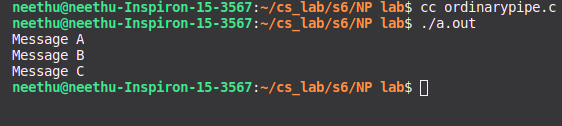
\includegraphics[scale=0.8]{img/e41.png}
\end{figure}
\subsubsection{Named Pipes}
\begin{verbatim}
// This side writes first, then reads
#include <stdio.h>
#include <string.h>
#include <fcntl.h>
#include <sys/stat.h>
#include <sys/types.h>
#include <unistd.h>

int main(){
    int fd;
    
    char * myfifo = "myfifo";
    
    mkfifo(myfifo, 0666);
    
    char arr1[80], arr2[80];
    while (1){
        	fd = open(myfifo, O_WRONLY);
        	fgets(arr2, 80, stdin);
        
        	write(fd, arr2, strlen(arr2)+1);
        	close(fd);
        
        	fd = open(myfifo, O_RDONLY);
        	read(fd, arr1, sizeof(arr1));
        
        	printf("User2: %s\n", arr1);
        	close(fd);
    }
    return 0;
}

// This side reads first, then writes
#include <stdio.h>
#include <string.h>
#include <fcntl.h>
#include <sys/stat.h>
#include <sys/types.h>
#include <unistd.h>

int main(){
    int fd1;
    
    char * myfifo = "myfifo";
    
    mkfifo(myfifo, 0666);
    
    char str1[80], str2[80];
    while (1){
        fd1 = open(myfifo,O_RDONLY);
        read(fd1, str1, 80);
        
        printf("User1: %s\n", str1);
        close(fd1);
        
        fd1 = open(myfifo,O_WRONLY);
        fgets(str2, 80, stdin);
        write(fd1, str2, strlen(str2)+1);
        close(fd1);
    }
    return 0;
}
\end{verbatim}
\begin{figure}[h]
            \centering
            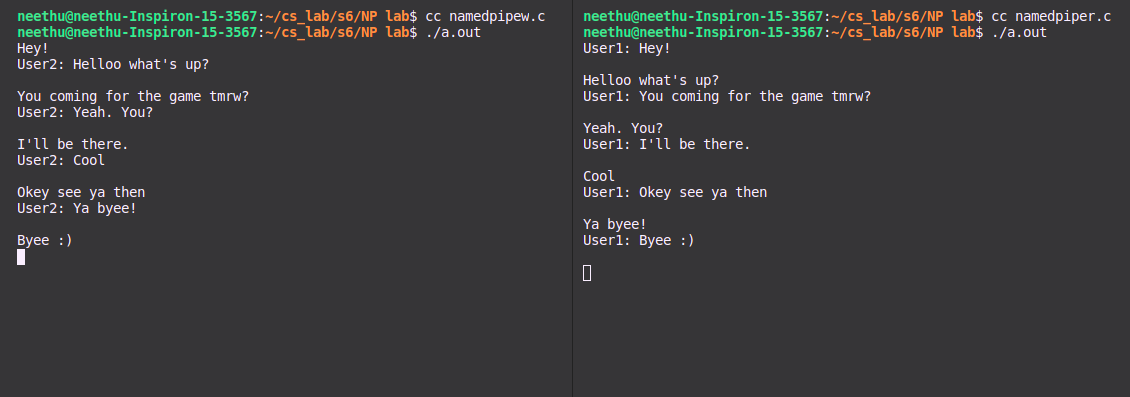
\includegraphics[scale=0.44]{img/e42.png}
\end{figure}

\subsubsection{Message Queue}
\begin{verbatim}
//Writer program
#include<stdio.h>
#include<sys/ipc.h>
#include<sys/msg.h>

struct msg_buffer{
    long msgType;
    char msgText[100];
}msg;

int main(){
    key_t key;
    int msgID;

    key = ftok("pgmfile", 65);
    msgID = msgget(key, 0666 | IPC_CREAT);
    msg.msgType = 1;

    printf("Write Data: ");
    scanf("%s",msg.msgText);
    msgsnd(msgID, &msg, sizeof(msg), 0);

    printf("Data sent is: %s\n", msg.msgText);
    return 0;
}

//Reader Program
#include<stdio.h>
#include<sys/ipc.h>
#include<sys/msg.h>

struct msg_buffer{
    long msgType;
    char msgText[100];
}msg;

int main(){
    key_t key;
    int msgID;

    key = ftok("pgmfile", 65);
    msgID = msgget(key, 0666 | IPC_CREAT);
    
    msgrcv(msgID, &msg, sizeof(msg), 1, 0);

    printf("Data received is: %s\n", msg.msgText);
    msgctl(msgID, IPC_RMID, NULL);
    
    return 0;
}
\end{verbatim}
\begin{figure}[h]
            \centering
            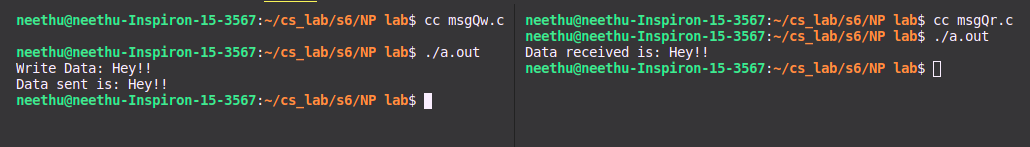
\includegraphics[scale=0.47]{img/e43.png}
\end{figure}

\subsubsection{Shared Memory}
\begin{verbatim}
//Writer Program
#include<sys/ipc.h>
#include<sys/shm.h>
#include<stdio.h>

int main(){
    key_t key = ftok("shmfile", 65);
    int shmID = shmget(key, 1024, 0666 | IPC_CREAT);
    char * str = (char *)shmat(shmID, (void *)0, 0);

    printf("Write Data: ");
    scanf("%s", str);
    printf("Data written in memory: %s\n", str);
    shmdt(str);

    return 0;
}

//Reader Program
#include<sys/ipc.h>
#include<sys/shm.h>
#include<stdio.h>

int main(){
    key_t key = ftok("shmfile", 65);
    int shmID = shmget(key, 1024, 0666 | IPC_CREAT);
    char * str = (char *)shmat(shmID, (void *)0, 0);

    printf("Data read from memory: %s\n", str);
    shmdt(str);
    shmctl(shmID, IPC_RMID, NULL);

    return 0;
}
\end{verbatim}
\begin{figure}[h]
            \centering
            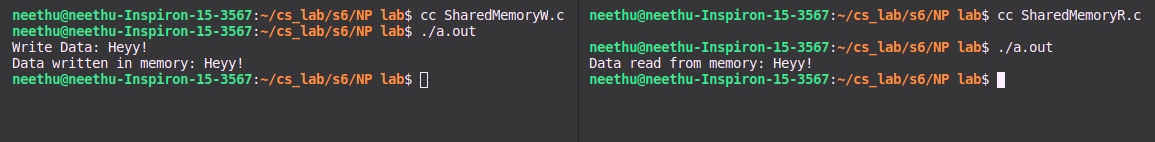
\includegraphics[scale=0.43]{img/e44.png}
\end{figure}

\subsection{Result}
Implemented the program for the inter-process communication using Pipes, Message Queues and Shared Memory using C language in Ubuntu 18.04 with kernel and the above outputs were obtained.

